\documentclass{article}
\setlength{\parskip}{0pt} % esp. entre parrafos
\setlength{\parindent}{3pt} % esp. al inicio de un parrafo
\usepackage{amsmath} % mates
\usepackage{listings}
\usepackage[sort&compress,numbers]{natbib} % referencias
\usepackage{url} % que las URLs se vean lindos
\usepackage[top=10mm,left=20mm,right=20mm,bottom=25mm]{geometry} % \textbf{\textbf{}}margenes
\usepackage{hyperref} % ligas de URLs
\usepackage{graphicx} % poner figuras
\usepackage[spanish]{babel} % otros idiomas
\hypersetup{
    colorlinks=true,
    linkcolor=blue,
    filecolor=blue,      
    urlcolor=blue,
    citecolor=black,
}

\title{TAREA \# 2 \\ Autómata celular} %titulo
\author{Natalia Berenice P\'{e}rez L\'{o}pez} % author
\date{\today}

\begin{document} % inicia contenido

\maketitle % cabecera

\section{Objetivo}
En esta práctica se trabaja con autómatas celulares en dos dimensiones, esto también se conoce como el "juego de la vida", el cual utiliza una sencilla regla de supervivencia: una celda está viva si exactamente tres vecinos suyos están vivos \citep{1}. El objetivo de esta práctica es determinar la probabilidad de creación de vida diseñando y ejecutando un experimento con por lo menos 30 réplicas en una malla de dimensión mayor o igual a diez, usando como límite de vida la supervivencia de 50 o más iteraciones en función de la probabilidad inicial de vida en por lo menos tres niveles diferentes entre 0 y 1. Al final se grafican y tabulan los hallazgos.

\section{Desarrollo} % seccion y etiqueta
Se realizaron diversos intentos para generar el código objetivo de la práctica, dichos intentos se encuentran en \href{https://github.com/nataliaperez0/Simulation/tree/main/Tarea2}{mi repositorio}  en GitHub. Se inició tomando como base el \href{https://github.com/satuelisa/Simulation/blob/master/CellularAutomata/gameOfLife.R}{código de autómata celular} revisado en clase para R \citep{2}. 

Las variables elegidas para ejecutar la práctica se muestran en el cuadro \ref{Cuadro 1}.

\begin{table}[ht]
\centering
\begin{tabular}{ |p{3cm}||p{3cm}|}
 \hline
 \multicolumn{2}{|c|}{Datos para el experimento} \\
 \hline
 Malla       & 18 X 18 \\
 \hline
 Replicas    & 40 \\
 \hline
 Iteraciones & 50 \\
 \hline
 Probabilidad inicial & 0.25, 0.50, 0.75 \\
 \hline
\end{tabular}
\caption{Datos del experimento 1.}
\label{Cuadro 1}
\end{table}

Primeramente al código base se le agregó la variable "p", la cual permite almacenar los tres niveles de probabilidad de población inicial (0.25, 0.50 y 0.75), posteriormente de acuerdo a las instrucciones dadas en clase se agregó un \texttt{for} para las probabilidades iniciales, dentro de él otro \texttt{for} para realizar la secuencia de replicas y dentro de este \texttt{for} se estableció el estado inicial del experimento, el cual cambiará al inicio de cada replica, seguido de esto se añadió la función que indica la regla de supervivencia para cada celda, y después mediante otro \texttt{for} se estableció la secuencia de iteraciones.
\bigskip

Para determinar si una replica crea vida infinita, se estableció que si existen celdas vivas después de 50 iteraciones la replica vivirá por siempre. De esta manera con una sentencia condicional \texttt{if} - \texttt{else} mi código contó como $vivos =1$ cada replica que sobrevivía el total de iteraciones, y contó como $vivos =0$ las replicas que morian al final de las 50 iteraciones o antes. Hasta este punto del diseño del código no se tenía ningún inconveniente, el problema se presentó al intentar sumar todas las replicas que generaban vida ($vivos =1$) y ordenarlas de acuerdo a la variable de probabilidad de población incial para después obtener un promedio de cada una de ellas.     
\bigskip

Con el fin de discutir y proponer posibles soluciones a este problema, se realizó una videollamada con mis compañeros Eduardo Navarro y Claudia Hernández. Después de intentar sin éxito algunas ideas para solucionar el problema que me tenía estancada, decidí intentar almacenar en un \texttt{data.frame} los $0$ y $1$ de cada replica por probabilidad inicial. Mi idea inicial era sumar en el \texttt{data.frame} los rangos de filas que pertenecían a cada probabilidad inicial y almacenar este dato en una variable, después dividir este dato entre el numero total de replicas y así obtener la probabilidad de generar vida infinita. Sin embargo, al revisar diferentes páginas de internet sobre documentación \citep{3,4} y video tutoriales \citep{5} para aprender a manipular datos de un \texttt{data.frame}, encontré una mejor opción. 

\newpage
.
\bigskip
\bigskip

La opción que encontré fue utilizar una función llamada \texttt{aggregate} \citep{6,7}, la cual permité agrupar datos que tengan una variable en común y realizar operaciones específicas con estos datos, de esta forma todos los $0$ y $1$ de la probabilidad inicial de $0.25$ se sumaron y se calculó su promedio automáticamente, lo mismo aplicó para las demás propabilidades iniciales. Este nuevo dato de promedio se almacenó en un segundo \texttt{data.frame} con su respectiva probabilidad inicial. 
\bigskip

Finalmente el último paso que se realizó fue gráficar el segundo \texttt{data.frame} generado,  para esto se utilizó la librería \texttt{ggplot2}. Se utilizó un tipo de gráfico de puntos para analizar la probabilidad inicial y su respectiva probabilidad de crear vida infinita, también se agregó una gráfica de línea suavizada para visualizar mejor el comportamiento de los datos. A continuación se muestra el código final para lograr el objetivo de la práctica y gráficar resultados:

\begin{lstlisting}[language=R]

library(parallel) #libreria para paralelizar
library(ggplot2) #libreria para graficar
library(dplyr) 
dim = 18 #dimension de la malla
num = dim^2
dur = 50 #numero de iteraciones
p = c(0.25, 0.50, 0.75) #probabilidades iniciales
datos1 = data.frame() #almacena los 0 y 1 de cada replica por prob. inicial
datos2 = data.frame() #almacena la prob. inicial y la prob. de vida infinita

for (inicial in p) { #para ejecutar las prob. iniciales
  for (replica in 1:40) { #para hacer replicas
    actual = matrix(round(runif(num) < p), nrow=dim, ncol=dim, byrow=TRUE)
    paso = function(pos) { #regla de superviviencia de las celdas
      fila = floor((pos - 1) / dim) + 1
      columna = ((pos - 1) %%  dim) + 1
      vecindad =  actual[max(fila - 1, 1) : min(fila + 1, dim), 
                         max(columna - 1, 1): min(columna + 1, dim)]
      return(1 * ((sum(vecindad) - actual[fila, columna]) == 3))
    }
    cluster <- makeCluster(detectCores(logical = FALSE) - 2)
    clusterExport(cluster, "dim")
    clusterExport(cluster, "paso")
    
    for (iteracion in 1:dur) { #para ejecutar 50 iteraciones
      clusterExport(cluster, "actual")
      siguiente <- parSapply(cluster, 1:num, paso)
      vivos = sum(siguiente)
      cat(inicial, replica, iteracion, vivos, '\n')
      actual <- matrix(siguiente, nrow=dim, ncol=dim, byrow=TRUE)
    }
    if (vivos > 0) {
      vivos = 1 #cuenta como 1 cuando la replica sobrevive 50 iteraciones
      print(vivos)
    } else {
      vivos = 0 #cuenta como 0 cuando la replica no sobrevive
      print(vivos)
    }
    vector = c(vivos) #vector que almacena todos los 0 y 1
    resultado = c(inicial, vivos) #almancena los 0 y 1 y su prob. inicial
    datos1 = rbind(datos1, resultado) #dataframe para 0, 1 y prob. inicial
    stopCluster(cluster)
  }
}

names(datos1) <- c("Prob", "Decision") #nombra las columnas del dataframe
datos2 = aggregate(Decision~Prob, datos1, mean) #promedio de prob. inicial
ggplot(datos2, aes(x= Prob, y= Decision)) + 
  geom_smooth(color="blue", size=1)+ #se puede cambiar a geom_line
  geom_point(shape=21, color="black", fill="#69b3a2", size=6)+
  theme_bw()+
  labs(x = "Probabilidad de poblacion inicial", y = "Probabilidad de vida infinita", 
  title = "Probabilidad de creacion de vida")

\end{lstlisting}

\section{Resultados y discusión}

En la figura \ref{Figura1} se muestra la gráfica resultante de los datos del experimento 1 proporcionados en el cuadro \ref{Cuadro 1}. 

\begin{figure} [h!]% figura
    \centering
    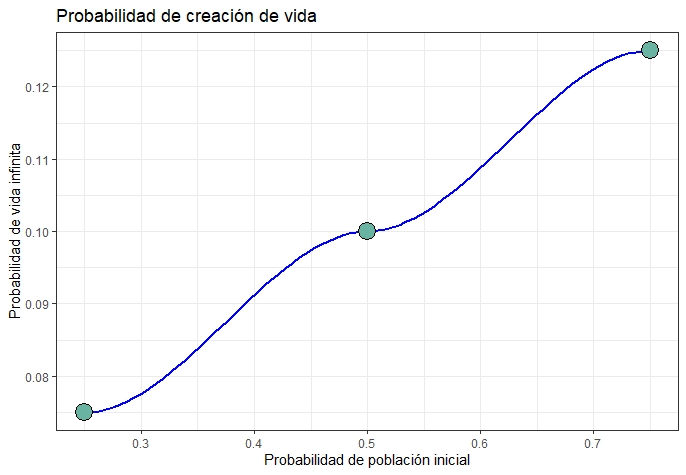
\includegraphics[width=150mm]{Figura1.jpeg} % archivo
    \caption{Gráfica que se obtiene al ejecutar el programa con los datos del experimento 1.}
    \label{Figura1}
\end{figure}

En la figura \ref{Figura1} podemos ver que la tendencia que sigue la gráfica es ascendente, de tal forma que cuando se tiene una mayor probabilidad de población inicial existe mayor probabilidad de crear vida infinita, sin embargo podemos notar en la gráfica y en el cuadro \ref{Cuadro 2} que el valor de la probabilidad de crear vida es realmente pequeño. 

\begin{table}[ht]
\centering
\begin{tabular}{ |p{3cm}||p{5cm}|}
 \hline
 Probabilidad inicial & Probabilidad de vida infinita\\
 \hline
 0.25 & 0.075 \\
 \hline
 0.50 & 0.100 \\
 \hline
 0.75 & 0.125 \\
 \hline
\end{tabular}
\caption{Resultados del experimento 1.}
\label{Cuadro 2}
\end{table}

A continuación se presentan los datos del experimento 2, en el cual se varían las probabilidades de población inicial y se conservan los demás parámetros del experimento 1 (Ver cuadro \ref{Cuadro 3}).

\newpage
.
\bigskip

\begin{table}[ht]
\centering
\begin{tabular}{ |p{3cm}||p{5cm}|}
 \hline
 \multicolumn{2}{|c|}{Datos para el experimento} \\
 \hline
 Malla       & 18 X 18 \\
 \hline
 Replicas    & 40 \\
 \hline
 Iteraciones & 50 \\
 \hline
 Probabilidad inicial & 0.15, 0.30, 0.45, 0.60, 0.75, 0.90 \\
 \hline
\end{tabular}
\caption{Datos del experimento 2.}
\label{Cuadro 3}
\end{table}

En la figura \ref{Figura2} se muestra la gráfica resultante de los datos del experimento 2 proporcionados en el cuadro \ref{Cuadro 3}. 

\begin{figure} [h!]% figura
    \centering
    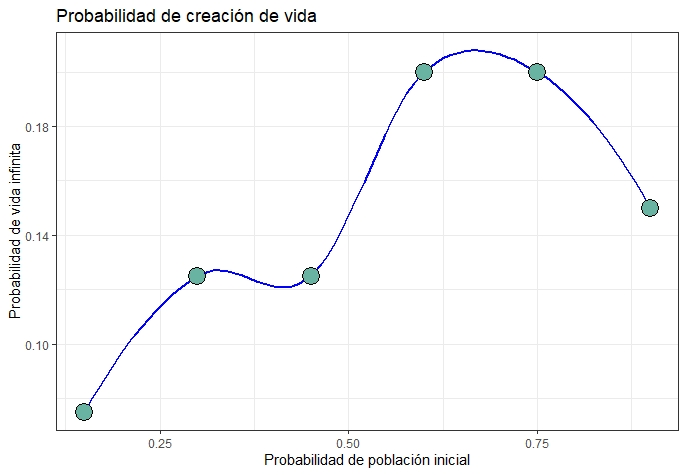
\includegraphics[width=150mm]{Figura2.jpeg} % archivo
    \caption{Gráfica que se obtiene al ejecutar el programa con los datos del experimento 2.}
    \label{Figura2}
\end{figure}

En la figura \ref{Figura2} podemos notar que la gráfica presenta un comportamiento ascendente con algunas zonas descendentes, sobre todo en las probabilidades de población inicial mayores de $0.75$ cercanas a $1$. En el cuadro \ref{Cuadro 4} se presentan los resultados númericos de la probabilidad de vida infinita para el experimento 2.

\begin{table}[ht]
\centering
\begin{tabular}{ |p{3cm}|p{4.5cm}||p{3cm}|p{4.5cm}|}
 \hline
 Probabilidad inicial & Probabilidad de vida infinita & Probabilidad inicial & Probabilidad de vida infinita\\
 \hline
 0.15 & 0.075 & 0.60 & 0.200 \\
 \hline
 0.30 & 0.125 & 0.75 & 0.200 \\
 \hline
 0.45 & 0.125 & 0.90 & 0.150 \\
 \hline
\end{tabular}
\caption{Resultados del experimento 2.}
\label{Cuadro 4}
\end{table}

Se puede observar que los datos del cuadro \ref{Cuadro 4} también representan probabilidades muy bajas de crear vida infinita en un mayor rango de probabilidades iniciales.
\bigskip

Enseguida se presentan los datos del experimento 3, en el cual se modifica la dimensión de la malla y se conservan los demás parámetros del experimento 1 (Ver cuadro \ref{Cuadro5}).
\newpage
.
\bigskip

\begin{table}[ht]
\centering
\begin{tabular}{ |p{3cm}||p{5cm}|}
 \hline
 \multicolumn{2}{|c|}{Datos para el experimento} \\
 \hline
 Malla       & 60 X 60 \\
 \hline
 Replicas    & 40 \\
 \hline
 Iteraciones & 50 \\
 \hline
 Probabilidad inicial & 0.25, 0.50, 0.75 \\
 \hline
\end{tabular}
\caption{Datos del experimento 3.}
\label{Cuadro5}
\end{table}

En la figura 3 se muestra la gráfica resultante de los datos del experimento 3 proporcionados en el cuadro \ref{Cuadro5}. 

\begin{figure} [h!]% figura
    \centering
    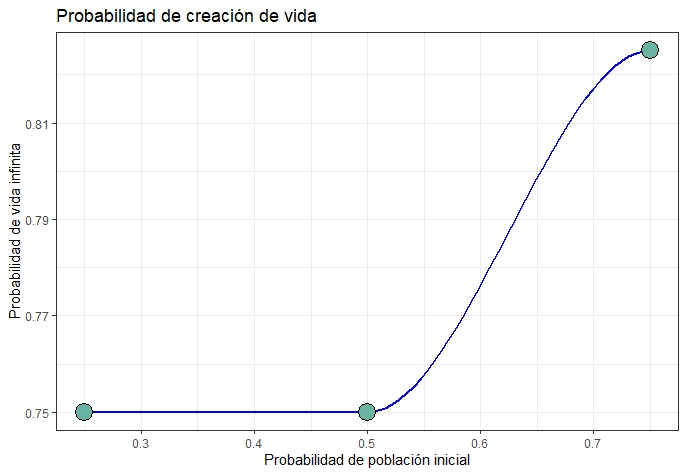
\includegraphics[width=150mm]{Figura3.jpeg} % archivo
    \caption{Gráfica que se obtiene al ejecutar el programa con los datos del experimento 3.}
    \label{Figura3}
\end{figure}

Su puede observar en la figura 3 que la gráfica presenta un comportamineto estable en probabilidades iniciales de $0.25$ y $0.50$ y un comportamiento ascendente cuando la probabilidad inicial aumenta a $0.75$, además podemos notar que los valores de la probabilidad de crear vida infinita son más grandes que los experimentos pasados con dimensiones de malla más pequeñas (Ver cuadro \ref{Cuadro 6}).

\begin{table}[ht]
\centering
\begin{tabular}{ |p{3cm}||p{5cm}|}
 \hline
 Probabilidad inicial & Probabilidad de vida infinita\\
 \hline
 0.25 & 0.750 \\
 \hline
 0.50 & 0.750 \\
 \hline
 0.75 & 0.825 \\
 \hline
\end{tabular}
\caption{Resultados del experimento 3.}
\label{Cuadro 6}
\end{table}

\bigskip
Como último experimento a continuación en el cuadro \ref{Cuadro7} se presentan los datos para el experimento 4, en cual se aumenta de nuevo la dimensión de la malla y se conservan los demás parámetros del experimento 1.

\newpage
.
\bigskip

\begin{table}[ht]
\centering
\begin{tabular}{ |p{3cm}||p{5cm}|}
 \hline
 \multicolumn{2}{|c|}{Datos para el experimento} \\
 \hline
 Malla       & 100 X 100 \\
 \hline
 Replicas    & 40 \\
 \hline
 Iteraciones & 50 \\
 \hline
 Probabilidad inicial & 0.25, 0.50, 0.75 \\
 \hline
\end{tabular}
\caption{Datos del experimento 4.}
\label{Cuadro7}
\end{table}

En la figura \ref{Figura 4} se muestra la gráfica resultante de los datos del experimento 4 proporcionados en el cuadro \ref{Cuadro7}. 

\begin{figure} [h!]% figura
    \centering
    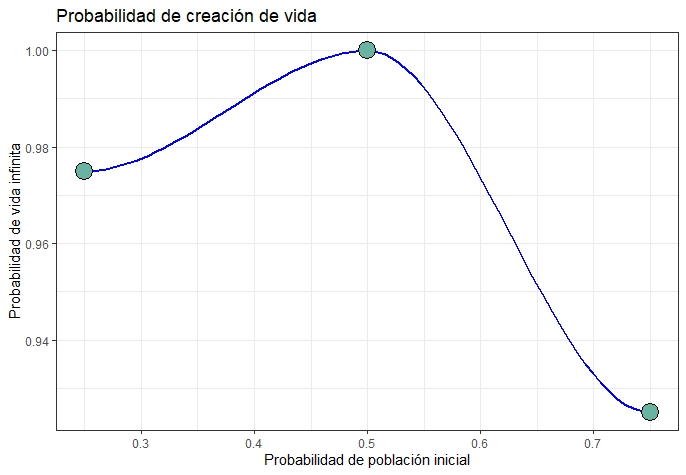
\includegraphics[width=150mm]{Figura4.jpeg} % archivo
    \caption{Gráfica que se obtiene al ejecutar el programa con los datos del experimento 4.}
    \label{Figura 4}
\end{figure}

En la figura \ref{Figura 4} podemos observar que el comportamiento de la gráfica es un poco distinto a la tendencia que presentaban los experimentos anteriores, sin embargo los valores de probabilidad de crear vida infinita son bastante grandes, además se observa que con una probabilidad inicial del $0.50$ la probabilidad de crear vida es de $1$, es decir que de 40 replicas realizadas, todas generaron vida (Ver cuadro \ref{Cuadro 8}).

\begin{table}[ht]
\centering
\begin{tabular}{ |p{3cm}||p{5cm}|}
 \hline
 Probabilidad inicial & Probabilidad de vida infinita\\
 \hline
 0.25 & 0.975 \\
 \hline
 0.50 & 1.00 \\
 \hline
 0.75 & 0.925 \\
 \hline
\end{tabular}
\caption{Resultados del experimento 4.}
\label{Cuadro 8}
\end{table}

Realizar los 4 experimentos me permitió analizar mejor de que depende mayormente la probabilidad de crear vida infinita en el código del "juego de la vida".

\newpage
.
\bigskip
\bigskip

\section{Conclusi\'{o}n}
Con base en los resultados que se muestran en las gráficas de las 4 figuras puedo concluir que la probabilidad de crear vida infinita depende mayormente de la dimensión de la malla, ya que cuando se tiene un tamaño mayor existe un rango más grande de espacio para la ejecución del programa, por lo que es más probable que el autómata celular pueda formar un patrón que le permita sobrevivir por siempre. Cuando se trata de dimensiones de malla pequeñas es muy poco probable que se forme un patrón que permita no morir. En cuanto a la probabilidad de población inicial considero que en la mayoría de los casos una mayor probabilidad inicial aumenta la probabilidad de crear vida infinita, sin embargo ésto no es un patrón que se repita en todas la ejecuciones del código. 

\bigskip

En general el desarrollo de la práctica me aportó más conocimiento sobe las funciones del programa RStudio y sobre como diseñar códigos.
\newpage
.
\bigskip
\bigskip

\bibliography{referencias}
\bibliographystyle{plainnat}

\end{document}